\documentclass[article]{jss}
\usepackage{amsfonts,hyperref}

%%%%%%%%%%%%%%%%%%%%%%%%%%%%%%
%% declarations for jss.cls %%
%%%%%%%%%%%%%%%%%%%%%%%%%%%%%%

%\usepackage{thumbpdf}

%% almost as usual
\author{David Meyer\\Wirtschaftsuniversit{\"a}t Wien \And
        Kurt Hornik\\Wirtschaftsuniversit{\"a}t Wien}
\title{Generalized and Customizable Sets in {\sf R}}

%% for pretty printing and a nice hypersummary also set:
\Plainauthor{David Meyer, Kurt Hornik} %% comma-separated

%% an abstract and keywords
\Abstract{
We present data structures and algorithms for
sets and some generalizations thereof (fuzzy
sets, multisets, and fuzzy multisets) available for {\sf R} through the
\pkg{sets} package. Fuzzy (multi-)sets are based on dynamically bound fuzzy
logic families. Further extensions include user-definable iterators
and matching functions.
}

\Keywords{\R, set, fuzzy logic, multiset, fuzzy set}
\Plainkeywords{R, sets, fuzzy logic, fuzzy set, multiset}

%\VignetteIndexEntry{Generalized and Customizable Sets in R}
%\VignetteDepends{sets}
%\VignetteKeywords{R, sets, fuzzy logic, fuzzy set, multiset}
%\VignettePackage{sets}

%% publication information
%% NOTE: This needs to filled out ONLY IF THE PAPER WAS ACCEPTED.
%% If it was not (yet) accepted, leave them commented.
%% \Volume{13}
%% \Issue{9}
%% \Month{September}
%% \Year{2004}
%% \Submitdate{2004-09-29}
%% \Acceptdate{2004-09-29}

%% The address of (at least) one author should be given
%% in the following format:
\Address{
  David Meyer\\
  Department of Information Systems and Operations\\
  E-mail: \email{David.Meyer@wu-wien.ac.at}\\
  URL: \url{http://wi.wu-wien.ac.at/~meyer/}\\

  Kurt Hornik\\
  Department of Statistics and Mathematics\\
  E-mail: \email{Kurt.Hornik@wu-wien.ac.at}\\
  URL: \url{http://statmath.wu-wien.ac.at/~hornik/}\\

  Wirtschaftsuniversit\"at Wien\\
  Augasse 2--6\\
  1090 Wien, Austria
}
%% It is also possible to add a telephone and fax number
%% before the e-mail in the following format:
%% Telephone: +43/1/31336-5053
%% Fax: +43/1/31336-734

%% for those who use Sweave please include the following line (with % symbols):
%% need no \usepackage{Sweave.sty}


\setkeys{Gin}{width=0.7\textwidth}


\newcommand\R{\textsf{R}}
\newcommand{\var}[1]{\textit{\texttt{#1}}}
\newcommand{\data}[1]{\texttt{#1}}
\newcommand{\class}[1]{\textsf{#1}}

\newcommand{\comment}[1]{\begin{quote} COMMENT. #1\end{quote}}

%% \code without `-' ligatures
\def\nohyphenation{\hyphenchar\font=-1 \aftergroup\restorehyphenation}
\def\restorehyphenation{\hyphenchar\font=`-}
{\catcode`\-=\active%
  \global\def\code{\bgroup%
    \catcode`\-=\active \let-\codedash%
    \Rd@code}}
\def\codedash{-\discretionary{}{}{}}
\def\Rd@code#1{\texttt{\nohyphenation#1}\egroup}

\newcommand{\eqn}[1]{$#1$}
\newcommand{\codefun}[1]{\code{#1()}}
\newcommand{\codefunind}[1]{\codefun{#1}\index{\texttt{#1}}}
\newcommand{\codeind}[1]{\code{#1}\index{\texttt{#1}}}
\newcommand{\sQuote}[1]{`{#1}'}
\newcommand{\dQuote}[1]{``{#1}''}

%% end of declarations %%%%%%%%%%%%%%%%%%%%%%%%%%%%%%%%%%%%%%%%%%%%%%%

\begin{document}

%% include your article here, just as usual
%% Note that you should use the \pkg{}, \proglang{} and \code{} commands.

\section[Introduction]{Introduction}

Only few will deny the importance of sets and set theory, building the
fundamentals of modern mathematics. For theory-building typically
axiomatic approaches \citep[e.g.,][]{sets:zermelo:1908, sets:fraenkel:1922}
are used. However, even
the primal, ``naive'' concept of sets representing ``collections''
of distinct objects \citep{sets:cantor:1895} discarding order
and count information seems both natural and practical.
The main operation being ``is-element-of'', sets alone are of limited
\emph{practical} use---they most of the times serve as basic building blocks for
more complex structures such as relations and generalized sets. A
common way is to consider pairs $(X, m)$ with set $X$ (``Universe'')
and membership function
$m : X \rightarrow D$ mapping each member to its ``grade''. The subset
of $X$ of elements with non-zero membership is called ``support''.
In \emph{multisets}, elements may appear more than once, i.e., $D =
\mathbb{N}_0$ ($m$ is also called the multiplicity function). There are many
applications in computer science and other disciplines
\citep[For a survey, see, e.g.,][]{sets:singh+ibrahim+yohanna:2007}.
In statistics, multisets appear as frequency tables. \emph{Fuzzy sets}
have become quite popular since their introduction by
\cite{sets:zadeh:1965}. Here, the membership function maps into the
unit interval. An interesting characteristic of fuzzy sets is that
the actual behavior of set operations depends on the underlying
fuzzy logic employed, which can be chosen according to domain-specific
needs. Fuzzy sets are actively used in fields such as machine
learning, engineering and artificial intelligence.
\comment{Survey-Refs? Wie viele, welche Gebiete?}
\emph{Fuzzy multisets} \citep{sets:yager:1986}
combine both approaches by allowing
each element to map to more than one fuzzy membership grade, i.e., $D$ is
the power set of multisets over the unit interval. Examples for the
application of fuzzy multisets can be found in the field of information
retrieval \citep[e.g.,][]{sets:matthe+caluwe+tre:2006}.

The use of sets and variants thereof is common in modern general purpose
programming languages:  \proglang{Java} and \proglang{C++}
provide corresponding abstract data types (ADTs) in their class
libraries, \proglang{Pascal} and \proglang{Python}
offer sets as native data type.
Surprisingly enough, sets are not standard in many
mathematical programming environments such as \proglang{Matlab} and
\proglang{Mathematica}, and also \R. Although the two latter offer
set operations such as union and intersection, these are applied to
ordered structures (lists and vectors, respectively),
\emph{interpreting} them as sets. When it comes to \R,
this emulation is far from complete, and occasionally leads to inconsistent
behavior. First of all, the existing infrastructure has no clear concept
of how to compare elements, leading to possibly confusing and
inconsistent behavior when different data types are involved in the
computations:
\begin{Schunk}
\begin{Sinput}
> s <- list(1, "1")
> union(s, s)
\end{Sinput}
\begin{Soutput}
[[1]]
[1] 1

[[2]]
[1] "1"
\end{Soutput}
\begin{Sinput}
> intersect(s, s)
\end{Sinput}
\begin{Soutput}
[[1]]
[1] 1
\end{Soutput}
\end{Schunk}
The reason is that most of the existing operations rely on
\codefun{match} which automatically performs type conversions
perturbing in this context.
Also, quite a few other basic operations such as
the Cartesian product, the power set, the subset predicate, etc., are
missing, let alone more specialized operations such as
the closure under union.
Then, the current facilities do not make use of a class
system, making extensions hard (if not impossible).  Another consequence
is that no distinction can be made between sequences (ordered
collections of objects) and sets (unordered collections of objects),
which is key for the definition of relations, where both concepts are
combined.  Also, there is no support for extensions such as fuzzy sets
or multisets.

We therefore implemented the \pkg{sets} package \citep{sets:meyer+hornik:2008}
presented here. The main goal was to provide a
flexible and customizable basic infrastructure for finite sets and the
generalizations mentioned above. As a side effect, the package
also provides basic operations for fuzzy logic. The remainder of the
paper is structured as follows. In Section \ref{sec:design}, we
discuss the design rationale of data structures and core algorithms.
Section \ref{sec:sets} introduces the most important set operations. Section
\ref{sec:gsets} starts with constructors and specific methods for
generalized sets, followed by a more focused presentation of the fuzzy
logic infrastructure. Section
\ref{sec:csets} shows how these can further be customized by specifying
user-definable matching functions and iterators. Section
\ref{sec:conclusion} concludes.

\section{Design issues}
\label{sec:design}

There are many ways of implementing sets. Choice and efficiency largely
depend on the domain range (i.e., the number of possible values for each
element). If the domain is relatively small, i.e. in the range of integral
data types such as \code{byte}, \code{integer}, \code{word} etc., the
probably most efficient representation is an array of bits
representing the domain elements like in \proglang{Pascal}
\citep{sets:wirth:1983}.
Operations such as union and
intersection can then straightforwardly be implemented
using logical \code{OR} and \code{AND}, respectively.
This approach obviously fails for intractably large domains
(e.g., strings or recursive objects). Without
further application knowledge, one needs to resort to generic
container ADTs with efficient element access such as hash tables or
search trees (for unique elements).
Operations can then be implemented following the classical
element-based definitions: Union by
inserting all elements of the smaller set into the
larger one; intersection by creating a new set with
all elements of the smaller set also contained in the larger one;
etc. Clearly, set comparison must be permutation invariant.
Some care is needed for nested structures (e.g., sets of sets of
\dots). Assume, e.g., the comparison of
$A = \{1, \{2, 3\}\}$ and $B = \{1, \{3, 2\}\}$ which clearly are identical.
A matching operator would need to check if, e.g., all elements of $A$ are
contained in $B$. If elements were internally stored in their order during
creation, the objects representing
$\{2, 3\}$ and $\{3, 2\}$ would be different. Comparing two set elements
for equality would thus require to recursively compare all elements
down the nested structures, which can quickly become unfeasible computationally.
This can be simplified by using a
canonical ordering during set creation,
guaranteeing that identical sets have identical
physical representation as well. We chose to sort
elements using their Unicode character representation, and to simply
store them in a list.
\comment{Mehr erkl{\"a}ren?}
For the sets package, further limitations are imposed by the
extensions presented in Sections \ref{sec:gsets} and
\ref{sec:csets}: Generalized sets require, for each element,
the membership information, and we also support user-defined, high-level
matching functions for comparing elements. Since operations defined
for generalized sets basically operate on the memberships,
it seems appropriate to store these as (generic) vectors.
Thus, memberships of
different sets can simply be combined element-wise.

A core operation is to match elements of two sets.
This is conceptionally
done by inserting the elements of the larger one into a hash
table (we use environments), and to look up the elements of the
smaller set in this table \citep[p.~391]{sets:knuth:1973}.
As hash key, we use the elements' character
representation. Since different objects can have the same
representation, we actually store the \emph{indices} of the elements in the
list, and match the actual objects using a simple linear search (Note that
since the element list is sorted, elements with same representation
are grouped, so the search will typically be fast).
Objects for sets, generalized sets and customizable sets have
\code{S3} classes \class{set}, \class{gset} and \class{cset},
respectively, with \class{set} inheriting from \class{gset} in turn
inheriting from \class{cset}. Accordingly, all operations have
\code{set\_} / \code{gset\_} / \code{cset\_} prefixes to give the user
the choice of up- or downcasts when objects of different class levels
are involved in one computation.
\comment{Kein {\"u}berzeugendes Argument: warum nicht generische
  Operatoren und casting via \code{as.\{c,g\}set}?}

\section{Sets}
\label{sec:sets}

The basic constructor for creating sets is the \codefunind{set}
function accepting an arbitrary number of \R{}~objects as arguments.
\begin{Schunk}
\begin{Sinput}
> s <- set(1L, 2L, 3L)
> print(s)
\end{Sinput}
\begin{Soutput}
{1L, 2L, 3L}
\end{Soutput}
\begin{Sinput}
> set("test", c, set("a", 2.5), list(1, 2))
\end{Sinput}
\begin{Soutput}
{"test", <<function>>, {"a", 2.5}, <<list(2)>>}
\end{Soutput}
\end{Schunk}
In addition, there is a generic \codefunind{as.set}
function coercing suitable objects to sets.
\begin{Schunk}
\begin{Sinput}
> s2 <- as.set(2:4)
> print(s2)
\end{Sinput}
\begin{Soutput}
{2L, 3L, 4L}
\end{Soutput}
\end{Schunk}
Elements can be named, allowing direct access and replacement
not possible otherwise.
\begin{Schunk}
\begin{Sinput}
> snamed <- set(one = 1, 2, three = 3)
> print(snamed)
\end{Sinput}
\begin{Soutput}
{one = 1, 2, three = 3}
\end{Soutput}
\begin{Sinput}
> snamed[["one"]]
\end{Sinput}
\begin{Soutput}
[1] 1
\end{Soutput}
\end{Schunk}
There are some basic predicate functions (and corresponding operators)
defined for the (in)equality, (proper) sub-(super-)set, and element-of
operations.
Note that all the \codefun{set\_is\_\var{foo}} functions are vectorized:
\begin{Schunk}
\begin{Sinput}
> set_is_empty(set())
\end{Sinput}
\begin{Soutput}
[1] TRUE
\end{Soutput}
\begin{Sinput}
> set_is_subset(set(1), set(1, 2))
\end{Sinput}
\begin{Soutput}
[1] TRUE
\end{Soutput}
\begin{Sinput}
> set(1) <= set(1, 2)
\end{Sinput}
\begin{Soutput}
[1] TRUE
\end{Soutput}
\begin{Sinput}
> set_contains_element(set(1, 2, 3), 1)
\end{Sinput}
\begin{Soutput}
[1] TRUE
\end{Soutput}
\begin{Sinput}
> 1:4 %e% set(1, 2, 3)
\end{Sinput}
\begin{Soutput}
[1] FALSE FALSE FALSE FALSE
\end{Soutput}
\end{Schunk}
Other than these predicate functions and operators, one can use:
\codefun{length} for the cardinality,
\codefun{c}, \code{|} and \code{+} for the union, \code{-} for the
difference (or complement), \code{\&} for the intersection,
\code{\%D\%} for the
symmetric difference, \code{*} and \code{\^{ }$n$} for the ($n$-fold)
Cartesian product (yielding a set of $n$-tuples), and \code{2\^} for the
power set.  \codefunind{set\_union}, \codefunind{set\_intersection}, and
\codefunind{set\_symdiff} accept more than two arguments.\footnote{The
  $n$-ary symmetric difference of a collection of sets consists of all
  elements contained in an odd number of the sets in the collection.}
\comment{Evtl. \code{+} und \code{-} nicht erw{\"a}hnen? Ist eigentlich
  direkte Summe und Differenz und macht f{\"u}r gsets was anderes.}
\begin{Schunk}
\begin{Sinput}
> ## cardinality
> length(s)
\end{Sinput}
\begin{Soutput}
[1] 3
\end{Soutput}
\begin{Sinput}
> ## complement, union, intersection, symmetric difference:
> s - 1L
\end{Sinput}
\begin{Soutput}
{2L, 3L}
\end{Soutput}
\begin{Sinput}
> s | set("a") + "b"
\end{Sinput}
\begin{Soutput}
{"a", "b", 1L, 2L, 3L}
\end{Soutput}
\begin{Sinput}
> s & s2
\end{Sinput}
\begin{Soutput}
{2L, 3L}
\end{Soutput}
\begin{Sinput}
> s %D% s2
\end{Sinput}
\begin{Soutput}
{1L, 4L}
\end{Soutput}
\begin{Sinput}
> ## Cartesian product
> s * s2
\end{Sinput}
\begin{Soutput}
{(1L, 2L), (1L, 3L), (1L, 4L), (2L, 2L), (2L, 3L), (2L, 4L), (3L, 2L),
 (3L, 3L), (3L, 4L)}
\end{Soutput}
\begin{Sinput}
> s ^ 2L
\end{Sinput}
\begin{Soutput}
{(1L, 1L), (1L, 2L), (1L, 3L), (2L, 1L), (2L, 2L), (2L, 3L), (3L, 1L),
 (3L, 2L), (3L, 3L)}
\end{Soutput}
\begin{Sinput}
> ## power set
> 2L ^ s
\end{Sinput}
\begin{Soutput}
{{}, {1L}, {2L}, {3L}, {1L, 2L}, {1L, 3L}, {2L, 3L}, {1L, 2L, 3L}}
\end{Soutput}
\end{Schunk}
\codefunind{set\_combn} returns the set of all subsets of specified
length. \codefun{closure} and \codefun{reduction} compute the closure
and reduction under union and intersection for set \emph{families}
(i.e., set of sets).
\begin{Schunk}
\begin{Sinput}
> set_combn(s, 2L)
\end{Sinput}
\begin{Soutput}
{{1L, 2L}, {1L, 3L}, {2L, 3L}}
\end{Soutput}
\begin{Sinput}
> cl <- closure(set(set(1), set(2), set(3)))
> print(cl)
\end{Sinput}
\begin{Soutput}
{{1}, {2}, {3}, {1, 2}, {1, 3}, {2, 3}, {1, 2, 3}}
\end{Soutput}
\begin{Sinput}
> reduction(cl)
\end{Sinput}
\begin{Soutput}
{{1}, {2}, {3}}
\end{Soutput}
\end{Schunk}
The \codefun{Summary} methods will also work if defined for the
elements:
\begin{Schunk}
\begin{Sinput}
> sum(s)
\end{Sinput}
\begin{Soutput}
[1] 6
\end{Soutput}
\begin{Sinput}
> range(s)
\end{Sinput}
\begin{Soutput}
[1] 1 3
\end{Soutput}
\end{Schunk}

Because set elements are unordered, it is not allowed to use positional
subscripting.  However, it is possible to iterate over \emph{all}
elements using \codefun{for} and \codefun{lapply}/\codefun{sapply}:
\begin{Schunk}
\begin{Sinput}
> sapply(s, sqrt)
\end{Sinput}
\begin{Soutput}
[1] 1.000000 1.414214 1.732051
\end{Soutput}
\begin{Sinput}
> for (i in s) print(i)
\end{Sinput}
\begin{Soutput}
[1] 1
[1] 2
[1] 3
\end{Soutput}
\end{Schunk}
Using \codefunind{set\_outer},
it is possible to apply a function on all factorial combinations of the
elements of two sets.  If only one set is specified, the function is
applied to all pairs of this set.
\begin{Schunk}
\begin{Sinput}
> set_outer(set(1, 2), set(1, 2, 3), "/")
\end{Sinput}
\begin{Soutput}
  1   2         3
1 1 0.5 0.3333333
2 2 1.0 0.6666667
\end{Soutput}
\end{Schunk}
\section{Generalized sets}
\label{sec:gsets}

There are several extensions of sets such as \emph{fuzzy sets}
and \emph{multisets}. Both can be be seen as special cases of
\emph{fuzzy multisets}. We present how they are constructed, and
demonstrate the effect of choosing different fuzzy logic families.

\subsection{Constructors and specific methods}

Generalized sets are created using the \codefun{gset} function,
expecting support and membership information. This
can be done in four ways:

\begin{enumerate}
\item Specify the support only (this yields a \dQuote{classical} set).
\item Specify support and memberships.
\item Specify support and membership function.
\item Specify a set of elements along with their individual membership grades.
\end{enumerate}

\noindent Note that for efficiency reasons, \codefun{gset} will not
store elements with zero memberships grades, i.e. really expects the
support and not a domain (or universe in the fuzzy world sense).
\begin{Schunk}
\begin{Sinput}
> X <- c("A", "B", "C")
> ## set (X is converted to a set internally).
> gset(support = X)
\end{Sinput}
\begin{Soutput}
{"A", "B", "C"}
\end{Soutput}
\begin{Sinput}
> ## multiset
> multi <- 1:3
> gset(support = X, memberships = multi)
\end{Sinput}
\begin{Soutput}
{"A" [1], "B" [2], "C" [3]}
\end{Soutput}
\begin{Sinput}
> ## fuzzy set
> ms <- c(0.1, 0.3, 1)
> gset(support = X, memberships = ms)
\end{Sinput}
\begin{Soutput}
{"A" [0.1], "B" [0.3], "C" [1]}
\end{Soutput}
\begin{Sinput}
> ## fuzzy set using a membership function
> f <- function(x) switch(x, A = 0.1, B = 0.2, C = 1, 0)
> gset(universe = X, charfun = f)
\end{Sinput}
\begin{Soutput}
{"A" [0.1], "B" [0.2], "C" [1]}
\end{Soutput}
\end{Schunk}
For fuzzy multisets,
the membership argument expects a list of membership grades,
either specified as vectors, or as multisets:
\begin{Schunk}
\begin{Sinput}
> ms2 <- list(c(0.1, 0.3, 0.4), c(1, 1), gset(support = ms, memberships = multi))
> gset(support = X, memberships = ms2)
\end{Sinput}
\begin{Soutput}
{"A" [{0.1, 0.3, 0.4}], "B" [{1 [2]}], "C" [{0.1 [1], 0.3 [2], 1 [3]}]}
\end{Soutput}
\end{Schunk}
As for sets, the usual operations
such as union, intersection, and complement are available.
Additionally, the sum and the difference of sets are defined,
which add and subtract multiplicities (or memberships for fuzzy sets):
\begin{Schunk}
\begin{Sinput}
> X <- gset(c("A", "B", "C"), 4:6)
> print(X)
\end{Sinput}
\begin{Soutput}
{"A" [4], "B" [5], "C" [6]}
\end{Soutput}
\begin{Sinput}
> Y <- gset(c("B", "C", "D"), 1:3)
> print(Y)
\end{Sinput}
\begin{Soutput}
{"B" [1], "C" [2], "D" [3]}
\end{Soutput}
\begin{Sinput}
> ## union vs. sum
> gset_union(X, Y)
\end{Sinput}
\begin{Soutput}
{"A" [4], "B" [5], "C" [6], "D" [3]}
\end{Soutput}
\begin{Sinput}
> gset_sum(X, Y)
\end{Sinput}
\begin{Soutput}
{"A" [4], "B" [6], "C" [8], "D" [3]}
\end{Soutput}
\begin{Sinput}
> ## intersection vs. difference
> gset_intersection(X, Y)
\end{Sinput}
\begin{Soutput}
{"B" [1], "C" [2]}
\end{Soutput}
\begin{Sinput}
> gset_difference(X, Y)
\end{Sinput}
\begin{Soutput}
{"A" [4], "B" [4], "C" [4]}
\end{Soutput}
\end{Schunk}

\subsection{Fuzzy logic and fuzzy sets}

For fuzzy (multi-)sets, the user can choose the logic underlying the
operations using the \codefun{fuzzy\_logic} function.  Fuzzy logics are
represented as named lists with four components \code{N}, \code{T},
\code{S}, and \code{I} containing the corresponding functions for
negation, conjunction (``t-norm''), disjunction (``t-conorm''), and
implication.  The fuzzy logic is selected by calling
\codefun{fuzzy\_logic} with a character string specifying the fuzzy
logic ``family'', and optional parameters. The exported functions
\codefun{.N.}, \codefun{.T.}, \codefun{.S.}, and \codefun{.I.} reflect
the currently selected bindings. Available families include:
\code{"Zadeh"} (default), \code{"drastic"}, \code{"product"},
\code{"Lukasiewicz"}, \code{"Fodor"}, \code{"Frank"}, \code{"Hamacher"},
\code{"Schweizer-Sklar"}, \code{"Yager"}, \code{"Dombi"},
\code{"Aczel-Alsina"}, \code{"Sugeno-Weber"}, \code{"Dubois-Prade"},
and \code{"Yu"} (see Appendix).  A call to
\codefun{fuzzy\_logic} without arguments returns the set fuzzy
logic currently set.

\begin{Schunk}
\begin{Sinput}
> x <- 1:10/10
> y <- rev(x)
> .S.(x, y)
\end{Sinput}
\begin{Soutput}
 [1] 1.0 0.9 0.8 0.7 0.6 0.6 0.7 0.8 0.9 1.0
\end{Soutput}
\begin{Sinput}
> fuzzy_logic("Fodor")
> .S.(x, y)
\end{Sinput}
\begin{Soutput}
 [1] 1 1 1 1 1 1 1 1 1 1
\end{Soutput}
\end{Schunk}
Fuzzy sets automatically use the fuzzy logic setting in
performing set operations:
\begin{Schunk}
\begin{Sinput}
> X <- gset(c("A", "B", "C"), c(0.3, 0.5, 0.8))
> print(X)
\end{Sinput}
\begin{Soutput}
{"A" [0.3], "B" [0.5], "C" [0.8]}
\end{Soutput}
\begin{Sinput}
> Y <- gset(c("B", "C", "D"), c(0.1, 0.3, 0.9))
> print(Y)
\end{Sinput}
\begin{Soutput}
{"B" [0.1], "C" [0.3], "D" [0.9]}
\end{Soutput}
\begin{Sinput}
> ## Zadeh-logic (default)
> fuzzy_logic("Zadeh")
> gset_intersection(X, Y)
\end{Sinput}
\begin{Soutput}
{"B" [0.1], "C" [0.3]}
\end{Soutput}
\begin{Sinput}
> gset_union(X, Y)
\end{Sinput}
\begin{Soutput}
{"A" [0.3], "B" [0.5], "C" [0.8], "D" [0.9]}
\end{Soutput}
\begin{Sinput}
> gset_complement(X, Y)
\end{Sinput}
\begin{Soutput}
{"B" [0.1], "C" [0.2], "D" [0.9]}
\end{Soutput}
\begin{Sinput}
> !X
\end{Sinput}
\begin{Soutput}
{"A" [0.7], "B" [0.5], "C" [0.2]}
\end{Soutput}
\begin{Sinput}
> ## switch logic to Fodor
> fuzzy_logic("Fodor")
> gset_intersection(X, Y)
\end{Sinput}
\begin{Soutput}
{"C" [0.3]}
\end{Soutput}
\begin{Sinput}
> gset_union(X, Y)
\end{Sinput}
\begin{Soutput}
{"A" [0.3], "B" [0.5], "C" [1], "D" [0.9]}
\end{Soutput}
\begin{Sinput}
> gset_complement(X, Y)
\end{Sinput}
\begin{Soutput}
{"D" [0.9]}
\end{Soutput}
\begin{Sinput}
> !X
\end{Sinput}
\begin{Soutput}
{"A" [0.7], "B" [0.5], "C" [0.2]}
\end{Soutput}
\end{Schunk}
The \codefun{cut} method for generalized sets
\dQuote{filters} all elements with membership
not less then a specified level---the result, thus, is a crisp (multi)set:
\begin{Schunk}
\begin{Sinput}
> cut(X, 0.5)
\end{Sinput}
\begin{Soutput}
{"B", "C"}
\end{Soutput}
\end{Schunk}
Additionally, there is a \codefun{plot} method for fuzzy (multi-)sets
that produces a barplot for the membership vector (see Figure \ref{fig:plot}):
\begin{Schunk}
\begin{Sinput}
> plot(X)
\end{Sinput}
\end{Schunk}

\begin{figure}[h]
\begin{center}
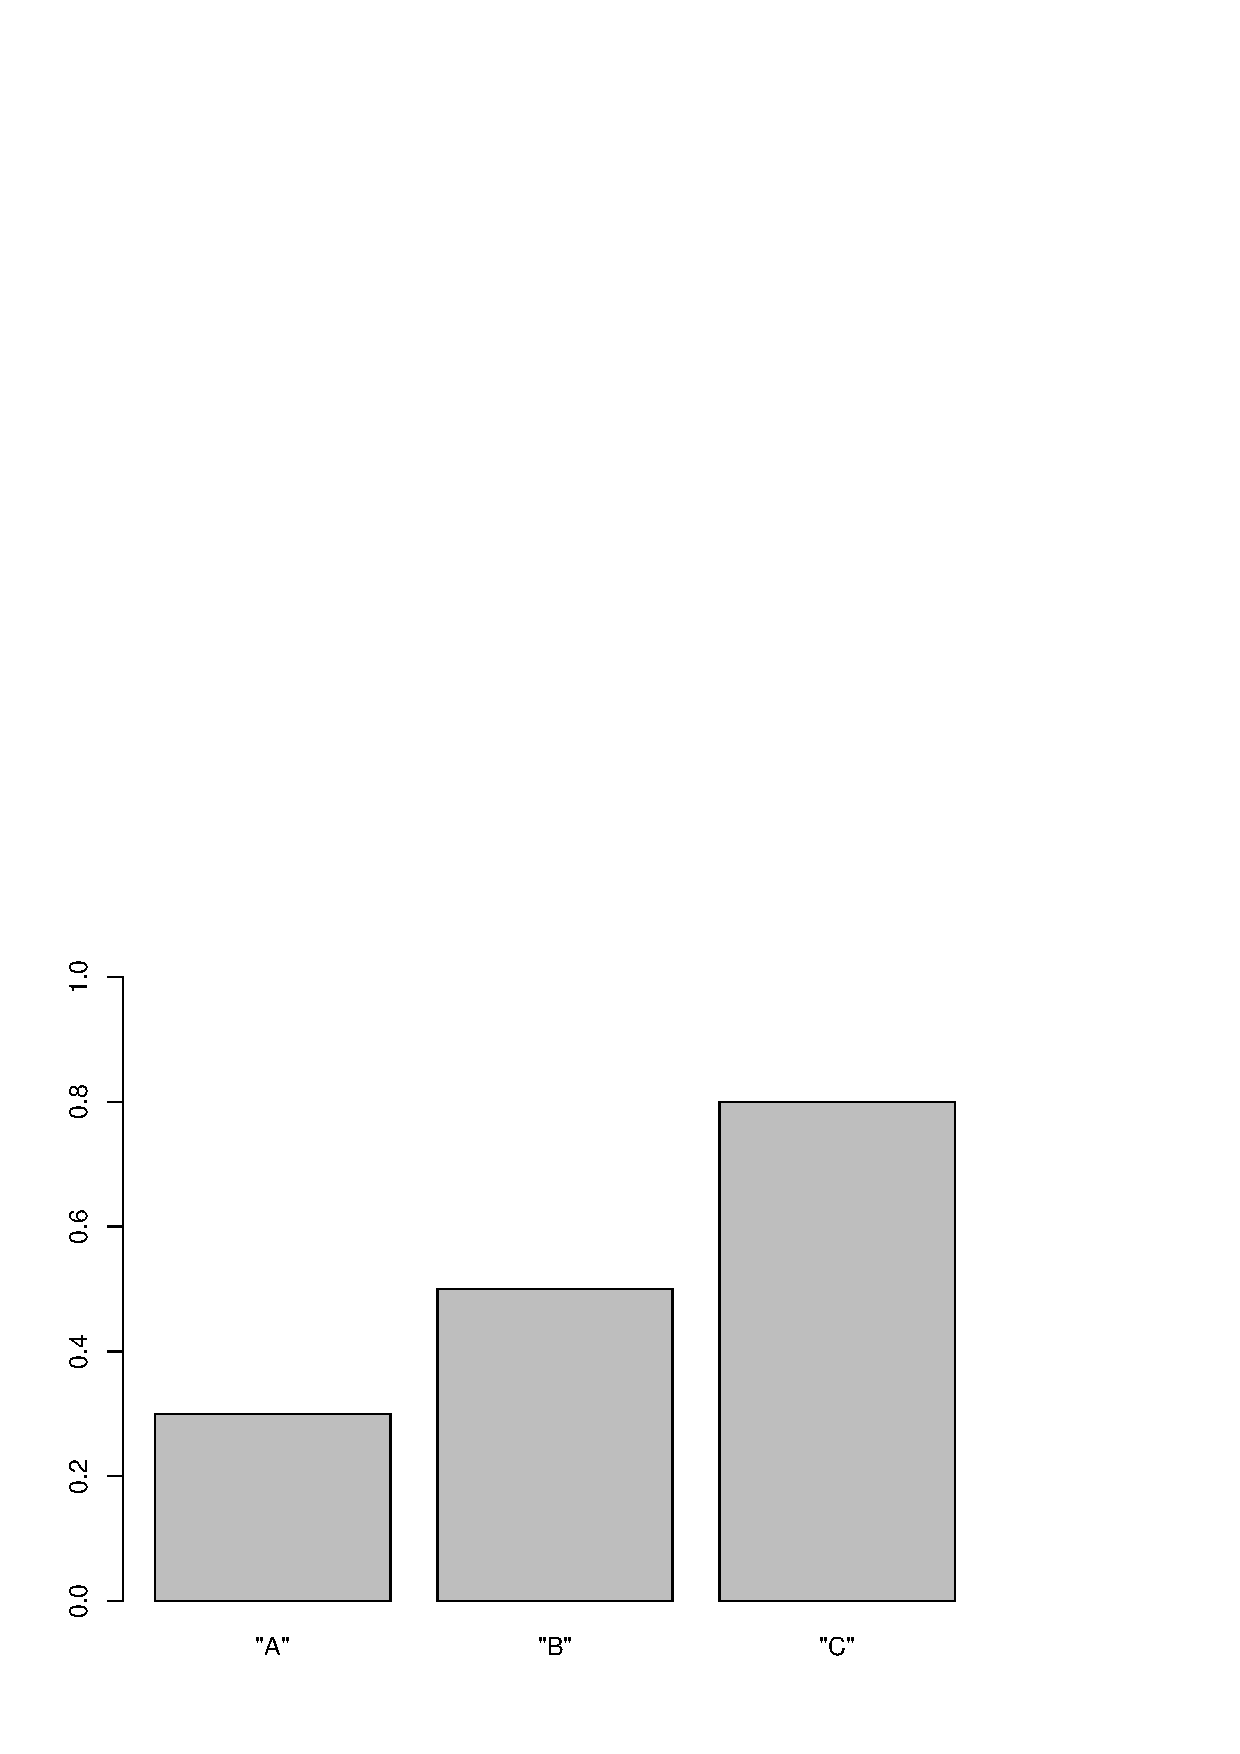
\includegraphics{JSS-020}
\caption{Membership plot for a fuzzy set.}
\label{fig:plot}
\end{center}
\end{figure}

\section{User-definable extensions}
\label{sec:csets}

We added \emph{customizable sets}
extending generalized sets in two ways: First, users
can control the way elements are matched, i.e., define equivalence
classes of elements. Second, arbitrary iteration orders can be specified.

\subsection{Matching functions}

By default, sets and generalized sets use
\codefun{identical} to match elements which is maximal
restrictive. Note that this differs from the behavior of
\code{"=="} or \codefun{match} which perform implicit type conversions
and thus confound, e.g., \code{1}, \code{1L} and \code{"1"}. In the
following example, note that on most computer systems, $3.3-2.2$ will not be
identical to $1.1$ due to numerical issues.
\begin{Schunk}
\begin{Sinput}
> x <- set("1", 1L, 1, 3.3 - 2.2, 1.1)
> print(x)
\end{Sinput}
\begin{Soutput}
{"1", 1L, 1, 1.1, 1.1}
\end{Soutput}
\begin{Sinput}
> y <- set(1, 1.1, 2L, "2")
> print(y)
\end{Sinput}
\begin{Soutput}
{"2", 2L, 1, 1.1}
\end{Soutput}
\begin{Sinput}
> 1L %e% y
\end{Sinput}
\begin{Soutput}
[1] FALSE
\end{Soutput}
\begin{Sinput}
> x | y
\end{Sinput}
\begin{Soutput}
{"1", "2", 1L, 2L, 1, 1.1, 1.1}
\end{Soutput}
\end{Schunk}
Customizable sets can be created using the \codefun{cset} constructor,
specifying the generalized set and some matching function.
\begin{Schunk}
\begin{Sinput}
> X <- cset(x, matchfun = match)
> print(X)
\end{Sinput}
\begin{Soutput}
{"1", 1.1}
\end{Soutput}
\begin{Sinput}
> Y <- cset(y, matchfun = match)
> print(Y)
\end{Sinput}
\begin{Soutput}
{"2", 1, 1.1}
\end{Soutput}
\begin{Sinput}
> 1L %e% Y
\end{Sinput}
\begin{Soutput}
[1] TRUE
\end{Soutput}
\begin{Sinput}
> X | Y
\end{Sinput}
\begin{Soutput}
{"1", "2", 1.1}
\end{Soutput}
\end{Schunk}
The specified \code{foo(x, table)} function needs to be vectorized in
the \code{table} argument. In order to make use of non-vectorized
predicates such as \codefun{all.equal}, the \pkg{sets} package
provides \codefun{make\_matchfun} to generate one:
\begin{Schunk}
\begin{Sinput}
> FUN <- make_matchfun(function(x, y) isTRUE(all.equal(x, y)))
> X <- cset(x, matchfun = FUN)
> print(X)
\end{Sinput}
\begin{Soutput}
{"1", 1L, 1.1}
\end{Soutput}
\begin{Sinput}
> Y <- cset(y, matchfun = FUN)
> print(Y)
\end{Sinput}
\begin{Soutput}
{"2", 2L, 1, 1.1}
\end{Soutput}
\begin{Sinput}
> 1L %e% Y
\end{Sinput}
\begin{Soutput}
[1] TRUE
\end{Soutput}
\begin{Sinput}
> X | Y
\end{Sinput}
\begin{Soutput}
{"1", "2", 1L, 2L, 1.1}
\end{Soutput}
\end{Schunk}
\noindent \codefunind{set\_options} can be used to conveniently switch the
default match and/or order function if a number of \class{cset} objects need
to be created:
\begin{Schunk}
\begin{Sinput}
> sets_options("matchfun", match)
> cset(x)
\end{Sinput}
\begin{Soutput}
{"1", 1.1}
\end{Soutput}
\begin{Sinput}
> cset(y)
\end{Sinput}
\begin{Soutput}
{"2", 1, 1.1}
\end{Soutput}
\begin{Sinput}
> cset(1:3) <= cset(c(1,2,3))
\end{Sinput}
\begin{Soutput}
[1] TRUE
\end{Soutput}
\end{Schunk}

\subsection{Iterators}

In addition to specifying matching functions, it is possible to
change the order in which
iterators such as \codefun{as.list}
\comment{But not for(), argh!}
process the elements. Note that the behavior of \codefun{as.list}
influences the labeling and print methods for
customizable sets. Sets and generalized sets by default
use the canonical internal ordering for iterations. With
customizable sets, a ``natural'' ordering of elements can be kept
by specifying either a permutation vector or an order function.

\begin{Schunk}
\begin{Sinput}
> cset(letters[1:5], orderfun = 5:1)
\end{Sinput}
\begin{Soutput}
{"e", "d", "c", "b", "a"}
\end{Soutput}
\begin{Sinput}
> FUN <- function(x) order(as.character(x), decreasing = TRUE)
> Z <- cset(letters[1:5], orderfun = FUN)
> print(Z)
\end{Sinput}
\begin{Soutput}
{"e", "d", "c", "b", "a"}
\end{Soutput}
\begin{Sinput}
> as.character(Z)
\end{Sinput}
\begin{Soutput}
[1] "a\n" "b\n" "c\n" "d\n" "e\n"
\end{Soutput}
\end{Schunk}
Note that converters for ordered factors keep the order:
\begin{Schunk}
\begin{Sinput}
> o <- ordered(c("a", "b", "a"), levels = c("b", "a"))
> as.set(o)
\end{Sinput}
\begin{Soutput}
{b, a}
\end{Soutput}
\begin{Sinput}
> as.cset(o)
\end{Sinput}
\begin{Soutput}
{a [1], b [2]}
\end{Soutput}
\end{Schunk}
Converters for other data types are order-preserving only
if elements are unique:
\begin{Schunk}
\begin{Sinput}
> as.cset(c("A", "quick", "brown", "fox"))
\end{Sinput}
\begin{Soutput}
{"A", "quick", "brown", "fox"}
\end{Soutput}
\begin{Sinput}
> as.cset(c("A", "quick", "brown", "fox", "quick"))
\end{Sinput}
\begin{Soutput}
{"A" [1], "brown" [1], "fox" [1], "quick" [2]}
\end{Soutput}
\end{Schunk}

\section{Conclusion}
\label{sec:conclusion}

In this paper, we described the \pkg{sets} package for \R, providing
infrastructure for sets and generalizations thereof such as fuzzy
sets, multisets and fuzzy multisets. The fuzzy variants make use of a
dynamic fuzzy logic infrastructure offering several fuzzy logic
families. Generalized sets are further extended to allow for
user-defined iterators and matching functions. Current work focuses on
data structures and algorithms for relations,
an important application of sets.

\begin{appendix}

\section{Available fuzzy logic families}
\label{sec:appendix}

  Let us
  refer to \eqn{N(x) = 1 - x} as the \emph{standard} negation, and,
  for a t-norm \eqn{T}, let \eqn{S(x, y) = 1 - T(1 - x, 1 - y)} be the
  \emph{dual} (or complementary) t-conorm.  Available specifications and
  corresponding families are as follows, with the standard negation used
  unless stated otherwise.
  \comment{Refs?}

  \begin{description}
    \item[\code{"Zadeh"}]{Zadeh's logic with \eqn{T = \min} and
      \eqn{S = \max}.  Note that the minimum t-norm, also known as the
      G{\"o}del t-norm, is the pointwise largest t-norm, and that the
      maximum t-conorm is the smallest t-conorm.}
    \item[\code{"drastic"}]{the drastic logic with t-norm
      \eqn{T(x, y) = y} if \eqn{x = 1}, \eqn{x} if \eqn{y = 1}, and 0
      otherwise, and complementary t-conorm \eqn{S(x, y) = y} if
      \eqn{x = 0}, \eqn{x} if \eqn{y = 0}, and 1 otherwise.  Note that
      the drastic t-norm and t-conorm are the smallest t-norm and
      largest t-conorm, respectively.}
    \item[\code{"product"}]{the family with the product t-norm
      \eqn{T(x, y) = xy} and dual t-conorm \eqn{S(x, y) = x + y - xy}.}
    \item[\code{"Lukasiewicz"}]{the Lukasiewicz logic with t-norm
      \eqn{T(x, y) = \max(0, x + y - 1)} and dual t-conorm
      \eqn{S(x, y) = \min(x + y, 1)}.}
    \item[\code{"Fodor"}]{the family with Fodor's \emph{nilpotent
	minimum} t-norm given by \eqn{T(x, y) = \min(x, y)} if
      \eqn{x + y > 1}, and 0 otherwise, and the dual t-conorm given by
    \eqn{S(x, y) = \max(x, y)} if \eqn{x + y < 1}, and 1 otherwise.}
    \item[\code{"Frank"}]{the family of Frank t-norms \eqn{T_p},
      \eqn{p \ge 0}, which gives the Zadeh, product and Lukasiewicz
      t-norms for \eqn{p = 0}, 1, and \eqn{\infty}, respectively,
      and otherwise is given by
      \eqn{T(x, y) = \log_p (1 + (p^x - 1) (p^y - 1) / (p - 1))}.}
    \item[\code{"Hamacher"}]{the three-parameter family of Hamacher,
      with negation \eqn{N_\gamma(x) = (1 - x) / (1 + \gamma x)},
      t-norm  \eqn{T_\alpha(x, y) = xy / (\alpha + (1 - \alpha)(x + y - xy))},
      and t-conorm
      \eqn{S_\beta(x, y) = (x + y + (\beta - 1) xy) / (1 + \beta xy)},
      where \eqn{\alpha \ge 0} and \eqn{\beta, \gamma \ge -1}.  This
      gives a deMorgan triple iff \eqn{\alpha = (1 + \beta) / (1 +
	\gamma)}.}
  \end{description}

  \noindent The following parametric families are obtained by combining the
  corresponding families of t-norms with the standard negation and
  complementary t-conorm.

  \begin{description}
  \item[\code{"Schweizer-Sklar"}]{the Schweizer-Sklar family
      \eqn{T_p}, \eqn{-\infty \le p \le \infty}, which
      gives the Zadeh (minimum), product and drastic t-norms for
      \eqn{p = -\infty}, \eqn{0}, and \eqn{\infty},
      respectively, and otherwise is given by
      \eqn{T_p(x, y) = \max(0, (x^p + y^p - 1)^{1/p})}.}
  \item[\code{"Yager"}]{the Yager family \eqn{T_p}, \eqn{p \ge 0},
      which gives the drastic and minimum t-norms for \eqn{p = 0}
      and \eqn{\infty}, respectively, and otherwise is given by
      \eqn{T_p(x, y) = \max(0, 1 - ((1-x)^p + (1-y)^p)^{1/p})}.}
  \item[\code{"Dombi"}]{the Dombi family \eqn{T_p}, \eqn{p \ge 0},
      which gives the drastic and minimum t-norms for \eqn{p = 0}
      and \eqn{\infty}, respectively, and otherwise is given by
      \eqn{T_p(x, y) = 0} if \eqn{x = 0} or \eqn{y = 0}, and
      \eqn{T_p(x, y) = 1 / (1 + ((1/x - 1)^p + (1/y - 1)^p)^{1/p})} if
      both \eqn{x > 0} and \eqn{y > 0}.}
  \item[\code{"Aczel-Alsina"}]{the family of t-norms \eqn{T_p},
      \eqn{p \ge 0}, introduced by Acz{\'e}l and Alsina, which gives the
      drastic and minimum t-norms for \eqn{p = 0} and
      \eqn{\infty}, respectively, and otherwise is given by
      \eqn{T_p(x, y) = \exp(-(|\log(x)|^p + |\log(y)|^p)^{1/p})}.}
  \item[\code{"Sugeno-Weber"}]{the family of t-norms \eqn{T_p},
      \eqn{-1 \le p \le \infty}, introduced by Weber
      with dual t-conorms introduced by Sugeno, which gives the
      drastic and product t-norms for \eqn{p = -1} and
      \eqn{\infty}, respectively, and otherwise is given by
      \eqn{T_p(x, y) = \max(0, (x + y - 1 + pxy) / (1 + p))}.}
  \item[\code{"Dubois-Prade"}]{the family of t-norms \eqn{T_p},
      \eqn{0 \le p \le 1}, introduced by Dubois and Prade, which gives
      the minimum and product t-norms for \eqn{p = 0} and \eqn{1},
      respectively, and otherwise is given by
      \eqn{T_p(x, y) = xy / \max(x, y, p)}.}
  \item[\code{"Yu"}]{the family of t-norms \eqn{T_p}, \eqn{p \ge -1},
      introduce by Yu, which gives the product and drastic t-norms for
      \eqn{p = -1} and \eqn{\infty}, respectively, and otherwise is
      given by \eqn{T(x, y) = \max(0, (1 + p) (x + y - 1) - p x y)}.}
  \end{description}

\end{appendix}

\bibliography{sets}

\end{document}
